\section{异构计算集群编程:CUDA stream 简介}
到目前为止,我们专注于对一台主机和一台设备的异构计算系统进行编程。 
在高性能计算(HPC)中,应用程序需要计算节点集群的聚合计算能力。 
如今,许多 HPC 集群的每个节点都有一台或多台主机和一台或多台设备。 
从历史上看,这些集群主要使用消息传递接口 (MPI) 进行编程。 在本章中,我们将介绍 MPI/CUDA 联合编程。 
我们将仅介绍程序员需要了解的 MPI 概念,以将其异构应用程序扩展到集群环境中的多个节点。 
特别是,我们将重点关注将 CUDA 内核扩展到多个节点的背景下的域分区、点对点通信和集体通信。

\subsection{背景}
尽管在 2009 年之前几乎没有顶级超级计算机使用 GPU,但对更高能源效率的需求导致近年来 GPU 的快速采用。 
当今世界上许多顶级超级计算机在每个节点中都使用 CPU 和 GPU。 
他们在 Green500 名单中的高排名验证了这种方法的有效性,这反映了他们的高能源效率。

当今计算集群的主导编程接口是 MPI(Gropp 等人,1999),它是一组 API 函数,用于计算集群中运行的进程之间的通信。 
MPI 采用分布式内存模型,其中进程通过相互发送消息来交换信息。 当应用程序使用API通信功能时,不需要处理互连网络的细节。 
MPI 实现允许进程使用逻辑号码相互寻址,这与在电话系统中使用电话号码的方式非常相似:电话用户可以使用电话号码互相拨打电话,
而无需确切知道被叫方的位置以及呼叫的路由方式。

\begin{figure}[H]
	\centering
	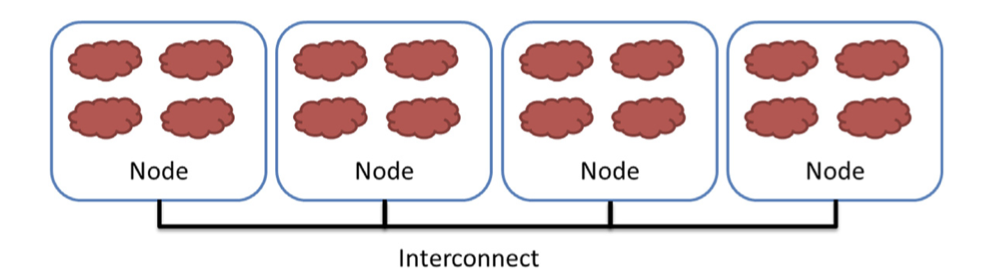
\includegraphics[width=0.9\textwidth]{figs/F20.1.png}
	\caption{\textit{程序员对 MPI 进程的看法。 MPI,消息传递接口。}}
\end{figure}

在典型的 MPI 应用程序中,数据和工作在进程之间划分。 
如图 20.1 所示,每个节点可以包含一个或多个进程,如图 20.1 所示,节点内显示为云。 
随着这些过程的进展,它们可能需要彼此的数据。 这种需求可以通过发送和接收消息来满足。 
在某些情况下,这些流程还需要在协作执行大型任务时相互同步并生成集体结果。 这是通过集体通信 API 函数完成的。

\subsection{一个运行的例子}
作为一个运行示例,我们将使用第 8 章“模板”中介绍的三维 (3D) 模板计算。 
我们假设计算基于有限差分法计算传热,用于求解描述传热物理定律的偏微分方程。 
特别是,我们将使用雅可比迭代方法,其中在每个迭代或时间步长中,
网格点的值被计算为邻居(北、东、南、西、上、下)及其自身的加权和 前一个时间步的值。 
为了实现高数值稳定性,在网格点的计算中还使用每个方向上的多个间接邻居。 
这是一个高阶模板计算,正如我们在第 8 章“模板”中讨论的那样。 为了本章的目的,我们假设每个方向将使用四个点。

\begin{figure}[H]
	\centering
	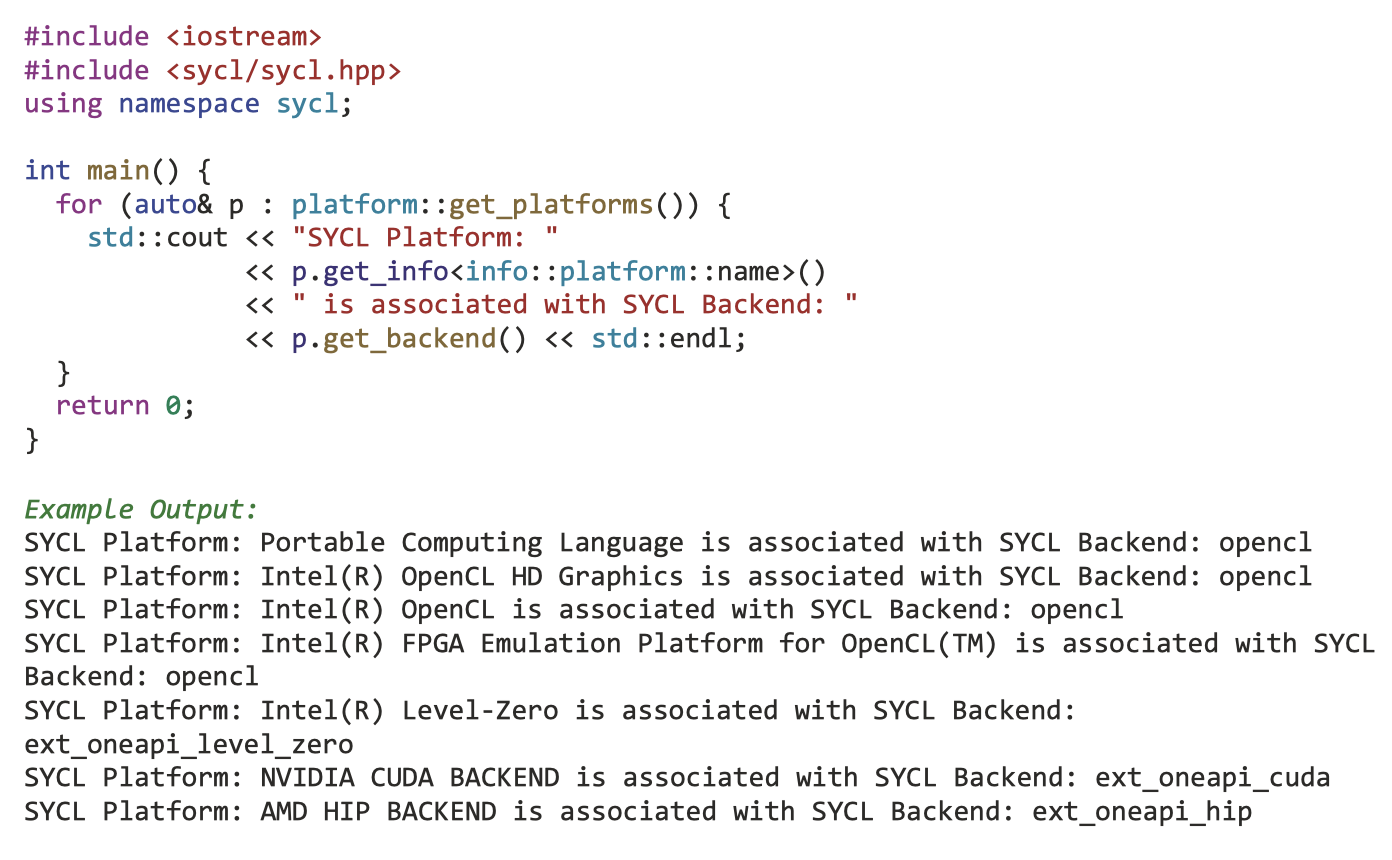
\includegraphics[width=0.9\textwidth]{figs/F20.2.png}
	\caption{\textit{25 点模板计算示例,x、y 和 z 方向各有四个邻居。}}
\end{figure}

如图20.2所示,一个网格点的下一步值的计算共有24个邻居点。 网格中的每个点都有 $x、y$ 和 $z$ 坐标。 
对于坐标值为$x=i、y=j$和$z=k$或($i$,$j,k)$的网格点,它的24个邻居是$(i-4,j) , k),(i-3, j, k),(i-2, j, k),(i-1, j, k),(i+$ $1, j, k),(i+2, j , k),(i+3, j, k),(i+4, j, k),(i, j-4, k),(i, j-3, k),(i, j-2 , k)$, $(i, j-1, k),(i, j+1, k),(i, j+2, k),(i, j+3, k),(i, j +4, k),(i, j, k-4),(i, j, k$ $-3),(i, j, k-2),(i, j, k-1),(i 、j、k+1)、(i、j、k+2)、(i、j、k+3)$ 和 $(i、j、k+$4)。 
由于下一个时间步的每个网格点的数据值是根据 25 个点(24 个邻居及其自身)的当前数据值计算的,因此这是一个 25 点模板计算。

\begin{figure}[H]
	\centering
	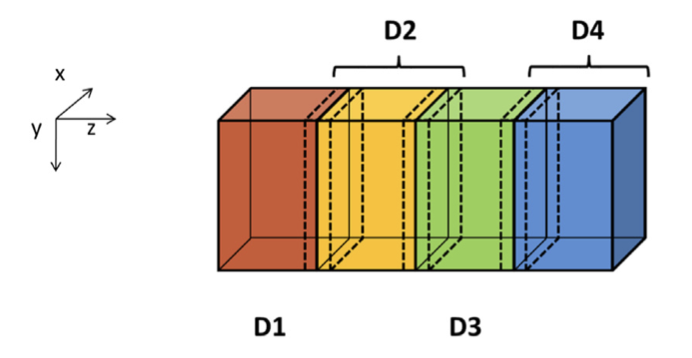
\includegraphics[width=0.9\textwidth]{figs/F20.3.png}
	\caption{\textit{用于对管道中的传热进行建模的 3D 网格阵列。}}
\end{figure}

我们假设系统被建模为结构化网格,其中网格点之间的间距在每个方向上都是恒定的。 
这允许我们使用 3D 数组,其中每个元素存储网格点的状态,正如我们在第 8 章“模板”中讨论的那样。 
每个维度中相邻元素之间的物理距离可以由网格间距变量来表示。 
请注意,此网格数据结构类似于第 18 章“静电势图”中静电势计算中使用的数据结构。 
图 20.3 展示了一个表示矩形通风管道的 3D 阵列,其中 $x$ 和 $y$ 尺寸为管道的横截面,$z$ 尺寸为沿管道的热流方向。

\begin{figure}[H]
	\centering
	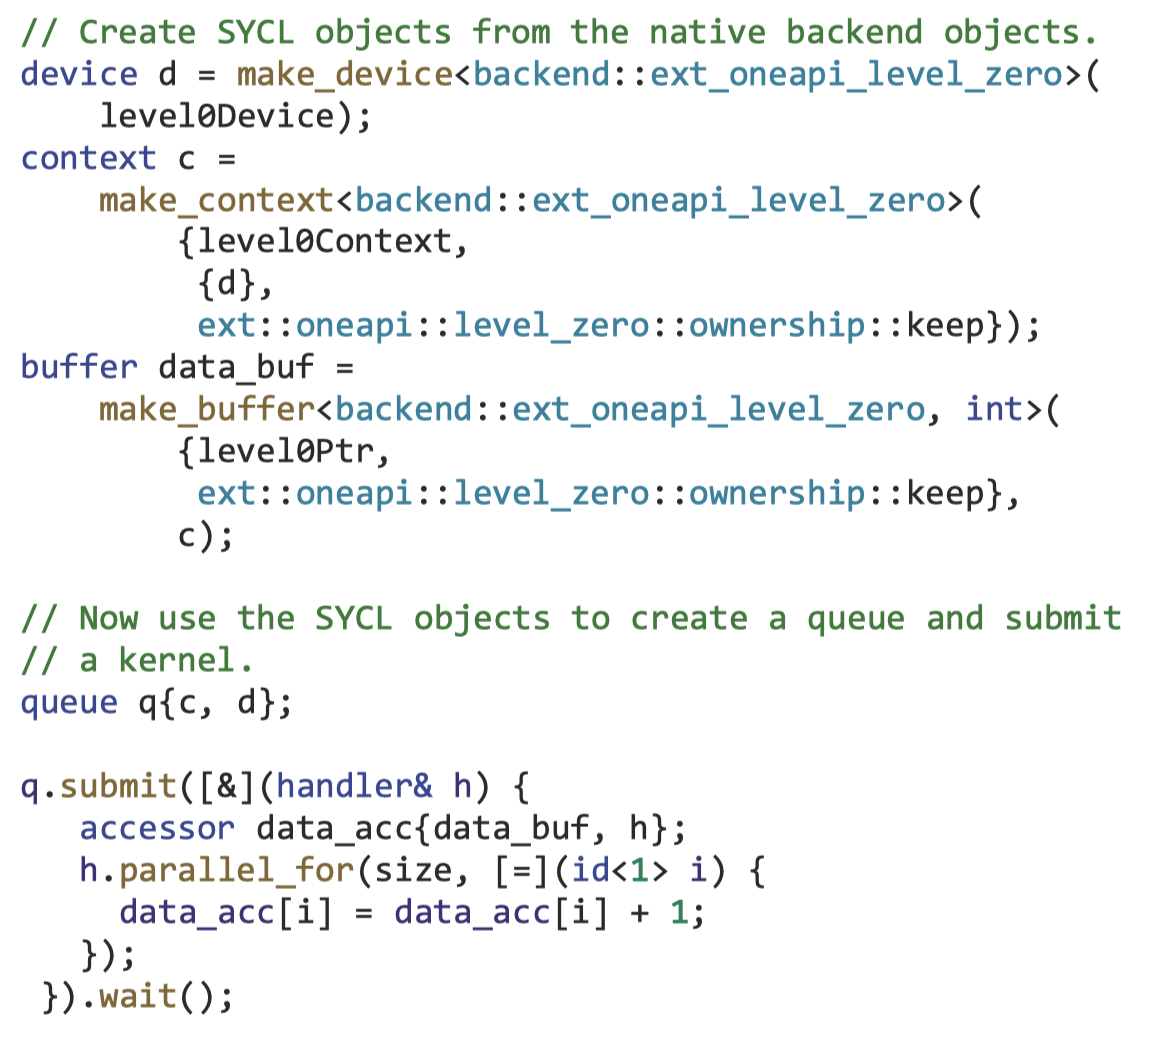
\includegraphics[width=0.9\textwidth]{figs/F20.4.png}
	\caption{\textit{3D 网格内存布局的一个小示例。}}
\end{figure}

我们假设数据以行优先布局放置在内存空间中,其中 $x$ 是最低维度,$y$ 是下一个维度,$z$ 是最高维度。 
也就是说,所有 $y=0$ 和 $z=0$ 的元素将根据其 $x$ 坐标放置在连续的内存位置中。 图 20.4 显示了网格数据布局的一个小例子。 
这个小示例在网格中只有 16 个数据元素:$x$ 维度中的两个元素,$y$ 维度中的两个元素,$z$ 维度中的四个元素。 
$y=0$ 和 $z=0$ 的 $x$ 元素首先放入内存中。 它们后面是所有 $y=1$ 和 $z=0$ 的元素。 
下一组将是 $y=0$ 和 $z=1$ 的元素。

当使用计算集群时,通常将输入数据划分为多个分区(称为域分区),并将每个分区分配给集群中的一个节点。 
在图 20.3 中,我们展示了 3D 数组被分为四个域分区:D0、D1、D2 和 D3。 每个分区都将分配给一个 MPI 计算进程。

域划分可以用图 20.4 进一步说明。 四个元素 $(z=0)$ 的第一个部分或切片位于第一个分区中; 
第二部分 $(z=1)$ 位于第二个分区中; 第三部分 $(z=2)$ 位于第三个分区中; 第四部分 $(z=3)$ 位于第四分区中。 
这显然是一个玩具示例。 在实际应用中,每个维度通常有数百甚至数千个元素。 
对于本章的其余部分,记住 $z$ 切片中的所有元素都位于连续的内存位置是有用的。

\subsection{消息传递接口基础知识}
\begin{figure}[H]
	\centering
	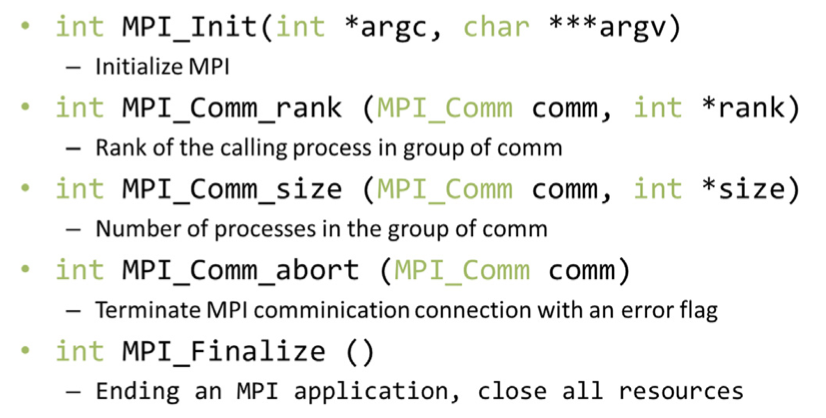
\includegraphics[width=0.9\textwidth]{figs/F20.5.png}
	\caption{\textit{用于建立和关闭通信系统的基本 MPI 功能。}}
\end{figure}

与 CUDA 一样,MPI 程序基于 SPMD 并行编程模型。 所有 MPI 进程都执行相同的程序。 
MPI系统提供了一组API函数来建立允许进程之间进行通信的通信系统。 
图 20.5 显示了为 MPI 应用程序建立和拆除通信系统的五个基本 MPI 功能。

\begin{figure}[H]
	\centering
	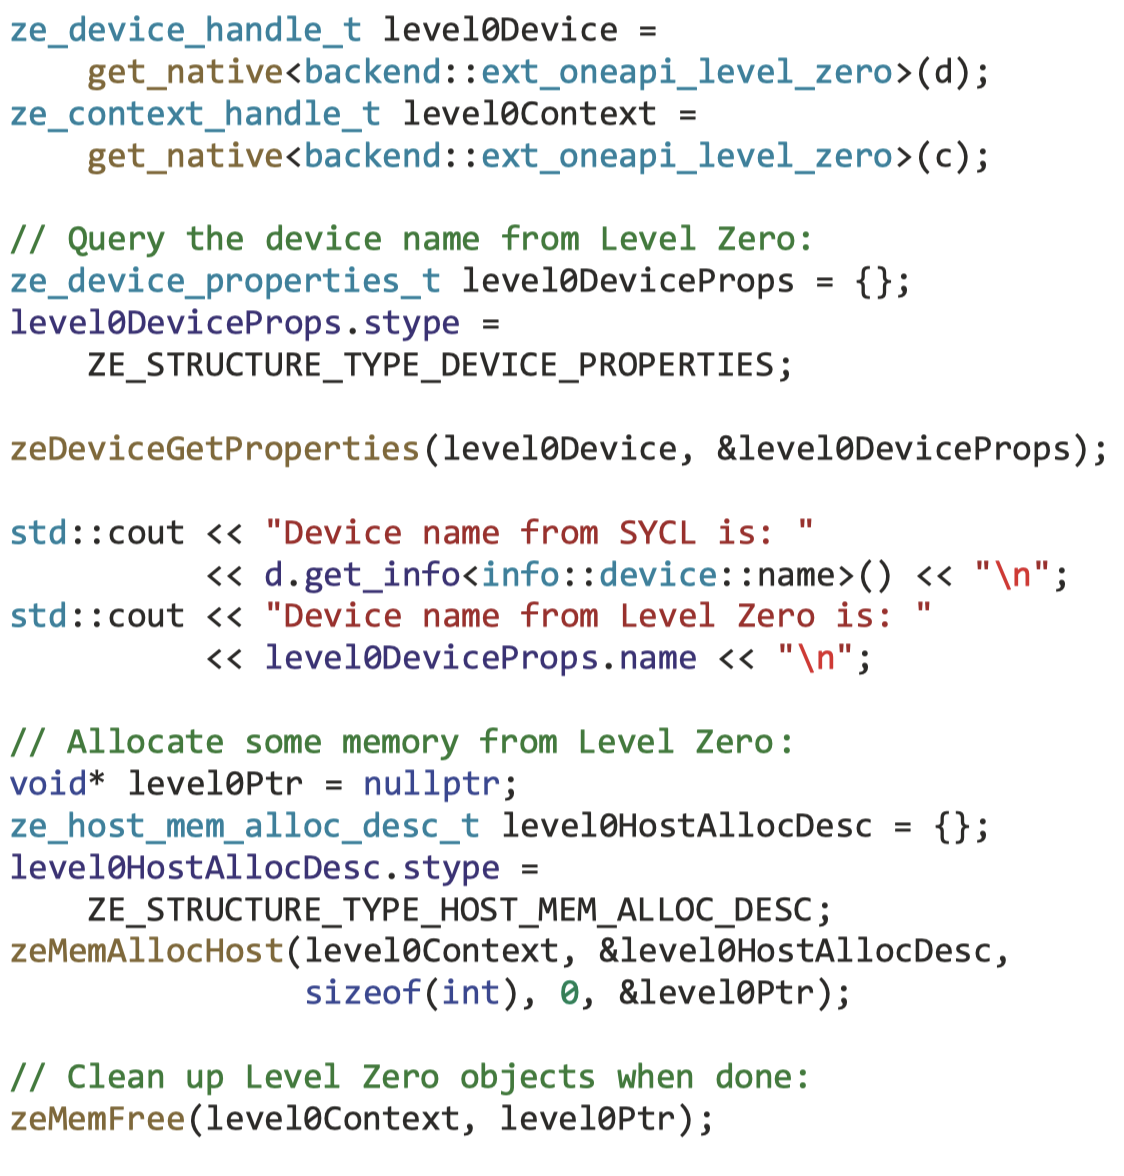
\includegraphics[width=0.9\textwidth]{figs/F20.6.png}
	\caption{\textit{一个简单的MPI主程序。}}
\end{figure}

我们将使用一个简单的 MPI 程序(如图 20.6 所示)来说明 API 函数的用法。 
要在集群中启动 MPI 应用程序,用户需要将程序的可执行文件提供给集群登录节点中的 mpirun 命令或 mpiexec 命令。 
每个进程首先通过 MPI\_Init() 调用(第 05 行)初始化 MPI 运行时。 这会初始化运行应用程序的所有进程的通信系统。 
一旦 MPI 运行时初始化,每个进程都会调用两个函数来准备通信。 
第一个函数是 MPI\_Comm\_rank()(第 06 行),它向每个调用进程返回一个唯一的编号,称为该进程的 MPI 等级或进程 ID。 
进程接收到的数字从 0 到进程数减 1 不等。 
进程的 MPI 等级类似于 CUDA 线程的表达式 blockIdx.x * blockDim.x+threadIdx.x。 
它唯一标识一次通信中的进程,也相当于电话系统中的电话号码。 
主要区别在于 MPI 等级是一维的。

图 20.6 第 06 行中的 MPI\_Comm\_rank () 函数有两个参数。
 第一个是 MPI 内置类型 MPI\_Comm,它指定请求的范围,即形成由 MIP\_Comm 变量标识的组的进程集合。 
 MPI\_comm 类型的每个变量通常称为通信器。 
 MPI\_Comm 和其他 MPI 内置类型在“mpi.h”头文件(第 01 行)中定义,所有使用 MPI 的 C 程序文件都应包含该头文件。 
 一个MPI应用程序可以创建一个或多个通信器,每个通信器都是一组用于通信目的的MPI进程。 
 MPI\_Comm\_rank() 为通信器中的每个进程分配一个唯一的 ID。 
 在图 20.6 中,传递的参数值是 MPI\_COMM\_WORLD,它用作默认值,意味着通信器包括正在运行应用程序的所有 MPI 进程。 
\footnote{有兴趣的读者应参阅 MPI 参考手册(Gropp et al., 1999),
了解有关在应用程序中创建和使用多个通信器的详细信息,特别是内部通信器和内部通信器的定义和使用。}

MPI\_Comm\_rank() 函数的第二个参数是一个指向整型变量的指针,函数将把返回的等级值存入该整型变量中。 
在图 20.6 中,为此目的声明了一个变量 pid。 MPI\_Comm\_rank() 返回后,pid 变量将包含调用进程的唯一 ID。

第二个 API 函数是 MPI\_Comm\_size( )(第 07 行),它返回通信器中运行的 MPI 进程总数。 
MPI\_Comm\_size() 函数有两个参数。 第一个是 MPI\_Comm 类型,给出请求的范围。 
图20.6中传入的参数值为MPI\_COMM\_WORLD,这意味着MPI\_Comm\_size()的作用范围是应用程序中的所有进程。 
由于范围是所有 MPI 进程,因此返回值是正在运行应用程序的 MPI 进程总数。 
该值由用户在使用 mpirun 命令或 mpiexec 命令执行应用程序时配置。 然而,用户可能没有请求足够数量的进程。 
此外,系统可能能够也可能无法创建用户请求的所有进程。 
因此,对于 MPI 应用程序来说,检查正在运行的进程的实际数量是一个很好的做法。

第二个参数是一个指向整型变量的指针,MPI\_Comm\_size() 函数将把返回值存入该变量。 
在图 20.6 中,为此目的声明了一个变量 np。 函数返回后,变量 np 包含正在运行应用程序的 MPI 进程数。 
在图 20.6 中,我们假设应用程序至少需要 3 个 MPI 进程。 因此它检查进程数是否至少为 3(第 08 行)。 
如果不是,则调用 MPI\_Comm\_abort() 函数终止通信连接并返回错误标志值 1(第 10 行)。

图 20.6 还显示了报告错误或其他琐事的常见模式。 MPI进程有多个,但我们只需要报错一次。 
应用程序代码指定 $\mathrm{pid}=0$ 的进程来执行报告(第 09 行)。 
这类似于 CUDA 内核中的模式,其中某些任务只需要由线程块中的一个线程来完成。

如图20.5所示,MPI\_Comm\_abort()函数有两个参数(第10行)。 第一个设置请求的范围。 
在图 20.6 中,范围设置为 MPI\_COMM\_WORLD,这意味着正在运行该应用程序的所有 MPI 进程。 
第二个参数是导致中止的错误类型的代码。 0 以外的任何数字都表示发生了错误。

如果进程数满足要求,则应用程序继续进行计算。 
在图 20.6 中,应用程序使用 np - 1 个进程( $\mathrm{pid}$ 从 0 到 $\mathrm{np}-2$ )来执行计算(第 12-13 行)
和一个进程(最后一个进程) 其 pid 为 $n p-1$ )为其他进程执行 I/O 服务(第 14-15 行)。 
我们将执行 I/O 服务的进程称为数据服务器,将执行计算的进程称为计算进程。 
在图20.6中,如果进程的pid在0到$\mathrm{np}-2$范围内,则它是一个计算进程并调用compute\_process()函数(第13行)。 
如果进程 pid 为 $n p-1$,则它是数据服务器并调用 data\_server() 函数(第 15 行)。 
这类似于线程根据其线程 ID 执行不同操作的模式。

应用程序完成计算后,它会调用 MPI\_Finalize() 来通知 MPI 运行时,这会释放分配给应用程序的所有 MPI 通信资源(第 16 行)。 
然后应用程序可以退出并返回值 0 ,这表示没有发生错误(第 17 行)。

\subsection{消息传递接口点对点通信}
MPI 支持两种主要类型的通信。 第一种是点对点类型,涉及一个源进程和一个目标进程。 
源进程调用 MPI\_Send() 函数,目标进程调用 MPI\_Recv() 函数。 这类似于电话系统中呼叫者拨打电话和接收者应答呼叫。

\begin{figure}[H]
	\centering
	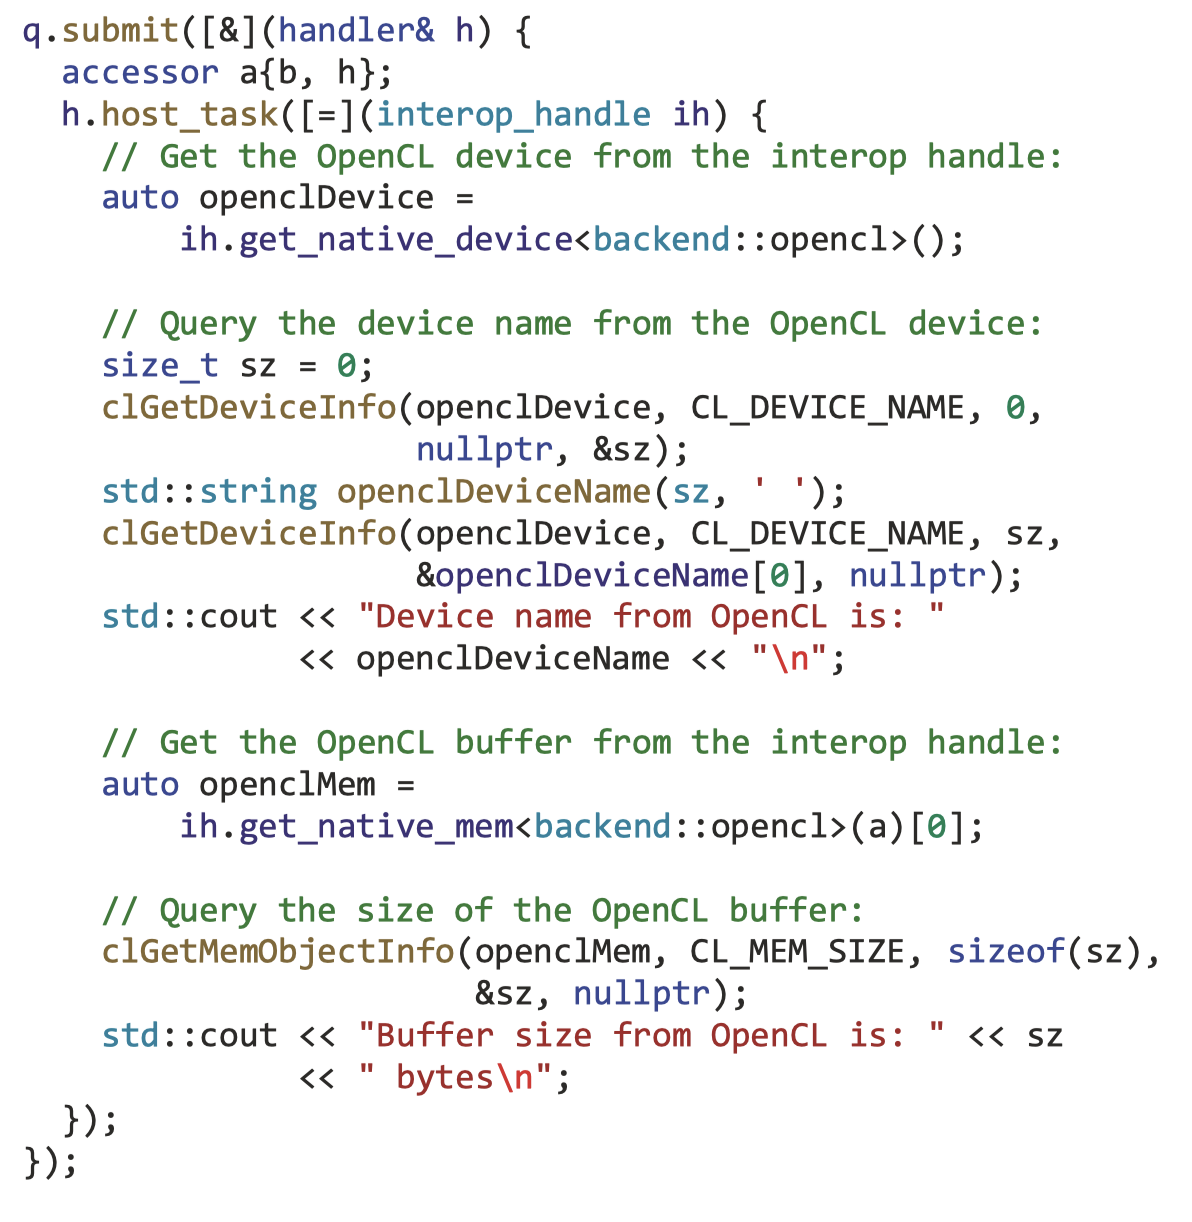
\includegraphics[width=0.9\textwidth]{figs/F20.7.png}
	\caption{\textit{MPI\_Send() 函数的语法。}}
\end{figure}

图 20.7 显示了使用 MPI\_Send( ) 函数的语法。 第一个参数是一个指针,指向可以找到要发送的数据的内存区域的起始位置。 
第二个参数是一个整数,给出要发送的数据元素的数量。 第三个参数是 MPI 内置类型 MPI\_Datatype。 
它指定就 MPI 库实现而言正在发送的每个数据元素的类型。 
MPI\_Datatype 的变量或参数可以保存的值在 mpi.h 中定义,包括 MPI\_DOUBLE(双精度浮点)、
MPI\_FLOAT(单精度浮点)、MPI\_INT(整数)和 MPI\_CHAR(字符)。 
这些类型的确切大小取决于主机处理器中相应的 $\mathrm{C}$ 类型的大小。 
有关 MPI 类型的更复杂的使用,请参阅 MPI 参考手册(Gropp 等人,1999)。

MPI\_Send( ) 的第四个参数是一个整数,给出目标进程的 MPI 等级。 
第五个参数给出一个标签,可用于对同一进程发送的消息进行分类。 第六个参数是指定定义目标 MPI 等级的上下文的通信器。

\begin{figure}[H]
	\centering
	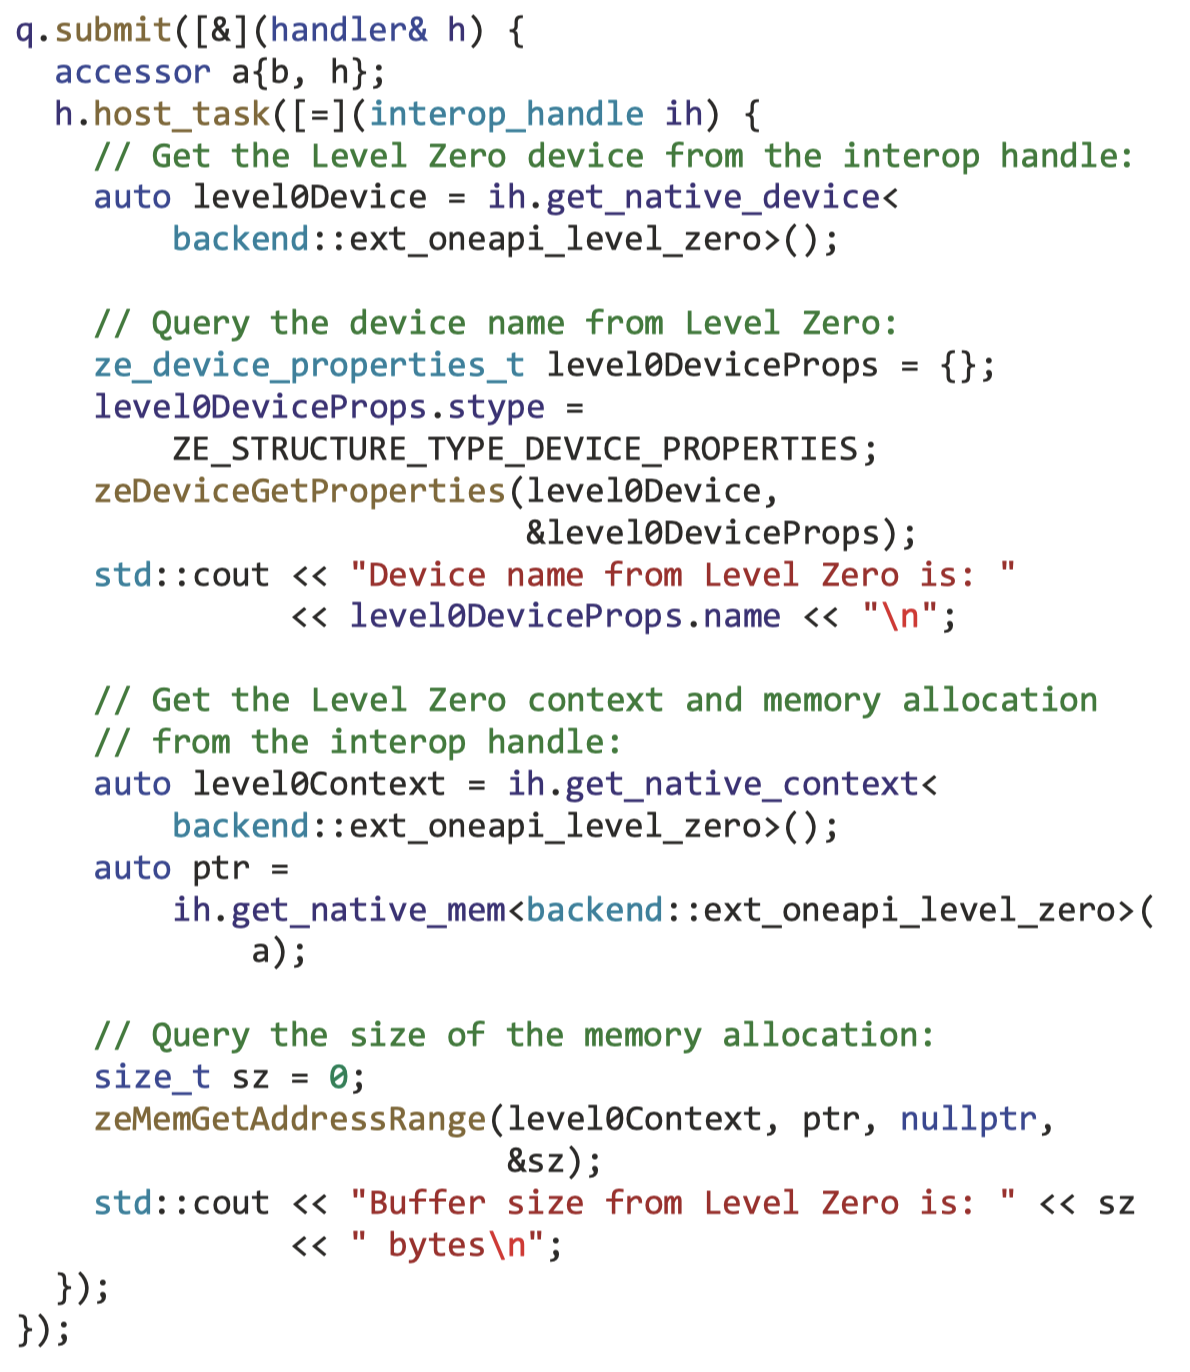
\includegraphics[width=0.9\textwidth]{figs/F20.8.png}
	\caption{\textit{MPI\_Recv() 函数的语法。}}
\end{figure}

图 20.8 显示了使用 MPI\_Recv( ) 函数的语法。 第一个参数是指向内存中应存放接收到的数据的区域的指针。 
第二个参数是一个整数,给出 MPI\_Recv() 函数允许接收的最大元素数。 
第三个参数是 MPI\_Datatype,它指定要接收的每个元素的类型。 第四个参数是一个整数,给出消息源的进程 ID。 
第五个参数是一个整数,指定目标进程期望的标记值。 
如果目标进程不希望被限制于特定的标记值,它可以使用MPI\_ANY\_TAG,这意味着接收者愿意接受来自源的任何标记值的消息。

我们首先使用数据服务器来说明点对点通信的使用。 在实际应用中,数据服务器进程通常会为计算进程执行数据输入和输出操作。 
然而,输入和输出具有太多依赖于系统的复杂性。 由于I/O不是我们讨论的重点,因此我们将避免集群环境中I/O操作的复杂性。 
也就是说,我们不需要从文件系统读取数据,而是让数据服务器用随机数初始化数据并将数据分发到计算进程。 
数据服务器代码的第一部分如图20.9所示。

数据服务器函数有四个参数。 前三个参数指定3D网格的大小:$x$维度中的元素数量,dimx; $y$ 维度中的元素数量,dimy; 
以及 $z$ 维度中的元素数量,dimz。 第四个参数指定网格中所有数据点需要完成的迭代次数。

\begin{figure}[H]
	\centering
	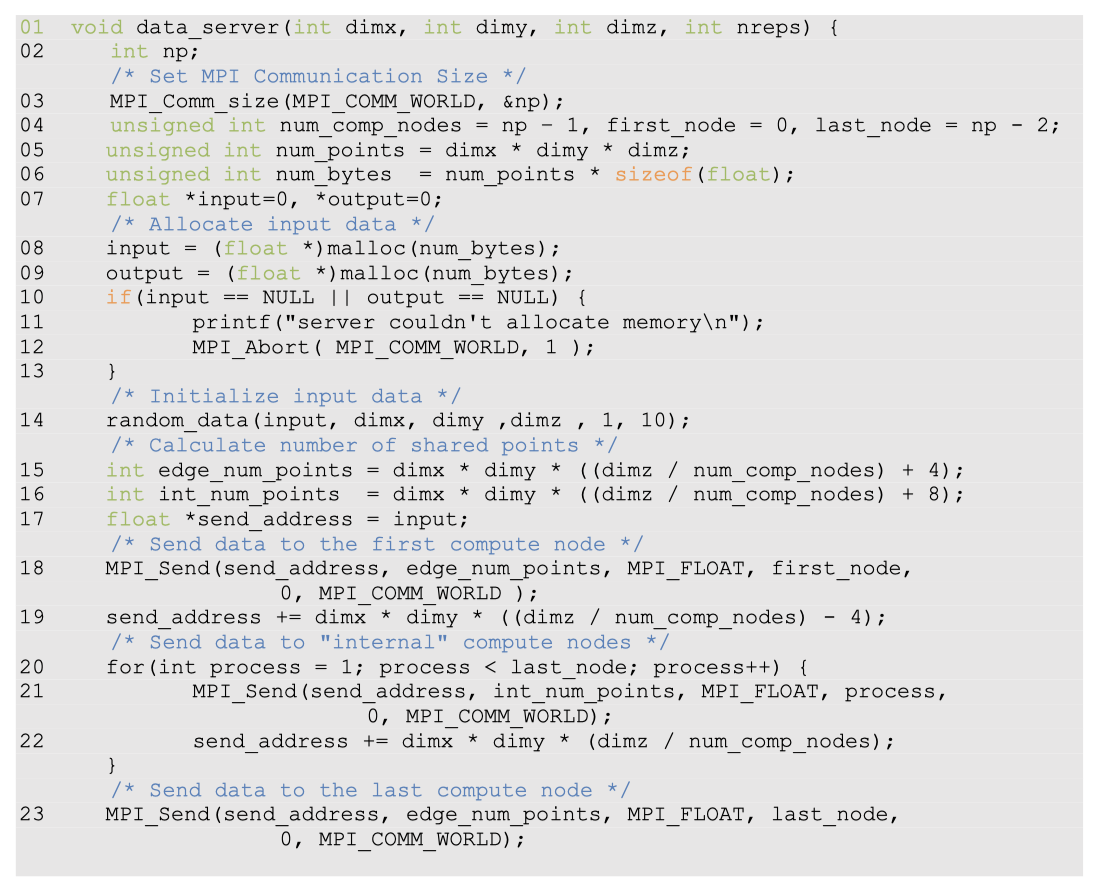
\includegraphics[width=0.9\textwidth]{figs/F20.9.png}
	\caption{\textit{数据服务器进程代码(第 1 部分)。}}
\end{figure}

在图 20.9 中,第 02 行声明了变量 np,它将包含运行应用程序的进程数。 
第 03 行调用 MPI\_Comm\_size( ),它将运行应用程序的进程数存入 np. 第 04 行声明并初始化了几个辅助变量。 
变量 num\_comp\_procs 包含计算进程的数量。 由于我们保留一个进程作为数据服务器,因此有 $n p-1$ 个计算进程。 
变量first\_proc给出第一个计算进程的进程ID,即0。 变量 1ast\_proc 给出最后一个计算进程的进程 ID,即 $n p-2$。 
也就是说,第 04 行将前 $n p-1$ 进程(0 到 $n p-2$)指定为计算进程。 排名最高的进程充当数据服务器。 
这反映了设计决策,并且该决策也将反映在计算过程代码中。

第05行声明并初始化了num\_points变量,该变量给出了要处理的网格数据点的总数,它只是每个维度中元素数量的乘积,
或dimx* dimy * dimz。 第 06 行声明并初始化 num\_bytes 变量,该变量给出了存储所有网格数据点所需的字节总数。 
由于每个网格数据点都是浮点数,因此该值为 num\_points* sizeof(float)。

第 07 行声明了两个指针变量:输入和输出。 这两个指针将指向输入数据缓冲区和输出数据缓冲区。 
第 08 行和第 09 行为输入和输出缓冲区分配内存,并将它们的地址分配给各自的指针。 第 10 行检查内存分配是否成功。 
如果任一内存分配失败,相应的指针将从 malloc() 函数接收到 NULL 指针。 
在这种情况下,代码会中止应用程序并报告错误(第 11-12 行)。

第 15 行和第 16 行计算应发送到每个计算进程的网格点数组元素的数量。 
如图20.3所示,有两种类型的计算进程:边缘进程和内部进程。 
第一个进程(进程 0,计算 D1)和最后一个进程(进程 3,计算 D4)计算仅在一侧具有邻居的边缘分区。 
分配给进程 0 的分区 D1 仅在右侧有一个邻居 (D2)。 分配给最后一个计算进程的分区 D4 仅在左侧 (D3) 有一个邻居。 
我们将计算边缘分区的计算过程称为边缘过程。 其他每个进程都会计算一个内部分区,该分区具有两种大小的邻居。 
例如,进程 1 计算分区 D2,它具有左邻居 (D1) 和右邻居 (D3)。 我们将计算内部分区的进程称为内部进程。

回想一下,在雅可比迭代方法中,网格点的每个计算步骤都需要上一步中其直接邻居的值。 
这就需要在分区的左右边界处设置网格点的光晕单元,这些网格点在图 20.3 中显示为由每个分区边缘的虚线定义的切片。 
请注意,这些光晕切片与第 8 章“模板”中介绍的模板图案中的光晕切片类似。 
由于我们正在计算每个方向有四个元素的 25 点模板,因此每个进程需要接收四个光环单元切片,
其中包含其分区边界网格点每一侧的所有邻居。 例如,在图20.3中,分区D2需要来自D1的四个光环切片和来自D3的四个光晕切片。 
请注意,D2 的光晕切片是 D1 或 D3 的边界切片。

回想一下,网格点的总数是 dimx * dimy * dimz。 
由于我们沿 $z$ 维度对网格进行分区,因此每个分区中的网格点数应为 dimx*dimy(dimz/num\_comp\_procs)。 
回想一下,我们在每个方向上需要四个相邻切片才能计算每个分区内的值。 
因此,应该发送到每个内部进程的网格点的数量是dimx*dimy((dimz/num\_comp\_procs)+8)。 
对于一个边缘进程来说,只有一个邻居。 与卷积的情况一样,我们假设零值将用于幽灵单元,并且不需要为它们发送输入数据。 
例如,分区 D1 仅需要右侧 D2 的四个相邻切片。 
因此,发送到边缘进程的网格点的数量为dimx*dimy((dimz/num\_comp\_procs)+4)。 
也就是说,每个进程从每侧的相邻分区接收四片光环网格点。

图 20.9 的第 17 行将 send\_address 指针设置为指向输入网格点数组的开头。 
为了将适当的分区发送到每个进程,我们需要为每个 MPI\_Send( ) 添加适当的偏移量到该起始地址。 我们稍后会回到这一点。

我们现在准备完成数据服务器的代码。 第 18 行向进程 0 发送其分区。 
由于这是第一个分区,因此它的起始地址也是整个网格的起始地址,这是在第17行设置的。进程0是边缘进程,它没有左邻居。 
因此要发送的网格点数量为值edge\_num\_points,即dimx*dimy((dimz/num\_comp\_procs)+4)。 
第三个参数指定每个元素的类型是 MPI\_FLOAT,即 C float(单精度,4 字节)。 
第四个参数指定first\_node的值,即0,是目标进程的MPI等级。 第五个参数指定 MPI 标记为 0。 
这是因为我们没有使用标签来区分从数据服务器发送的消息。 
第六个参数指定用于解释消息的发送方和接收方等级值的通信器应该是当前应用程序的所有 MPI 进程。

图 20.9 的第 19 行将 send\_address 指针前进到进程 1 的数据分区的开头。
从图 20.3 中,分区 D1 中有 dimx*dimy(dimz/num\_comp\_procs) 元素,
其中 表示 D2 从距离输入起始位置为 dimx*dimy(dimz/num\_comp\_procs) 个元素的位置开始。 
回想一下,我们还需要从 D1 发送光环单元。 因此,我们将 MPI\_Send( ) 的起始地址向后调整四个切片,
从而得到第 19 行中用于推进 send\_address 指针的表达式: dimx*dimy((dimz/num\_comp\_procs) - 4).

第 20 行是一个循环,它将 MPI 消息发送到内部进程(进程 1 到进程 $\mathrm{np}-3$ )。 
在我们的四个计算进程的小示例中,np 为 5,因此循环将 MPI 消息发送到进程 1 和进程 2。
这些内部进程需要接收两侧邻居的光环网格点。 因此第21行的MPI\_Send()的第二个参数使用int\_num\_nodes,
即dimx*dimy((dimz/num\_comp\_procs)+8)。 
其余参数与第 18 行中的 MPI\_Send() 类似,但明显的例外是目标进程由循环变量 process 指定,
该变量从 1 递增到 $n p-3$(last\_node 是 $n p-2$ )。

第 22 行将每个内部进程的发送地址前进每个分区中网格点的数量:dimx*dimy*dimz/num\_comp\_nodes。 
请注意,内部进程的光环网格点的起始位置是 dimx*dimy*dimz/ num\_comp\_procs 点相距。 
虽然我们需要将起始地址拉回四个切片来容纳光环网格点,但我们对每个内部进程都这样做,
因此起始位置之间的净距离仍然是每个分区中网格点的数量。

第 23 行将数据发送到进程 $n p-2$,这是左边只有一个邻居的最后一个计算进程。 读者应该能够推理出所使用的所有参数值。 
请注意,我们还没有完全完成数据服务器代码。 我们稍后将回来讨论数据服务器的最后部分,该部分收集所有计算进程的输出值。

\begin{figure}[H]
	\centering
	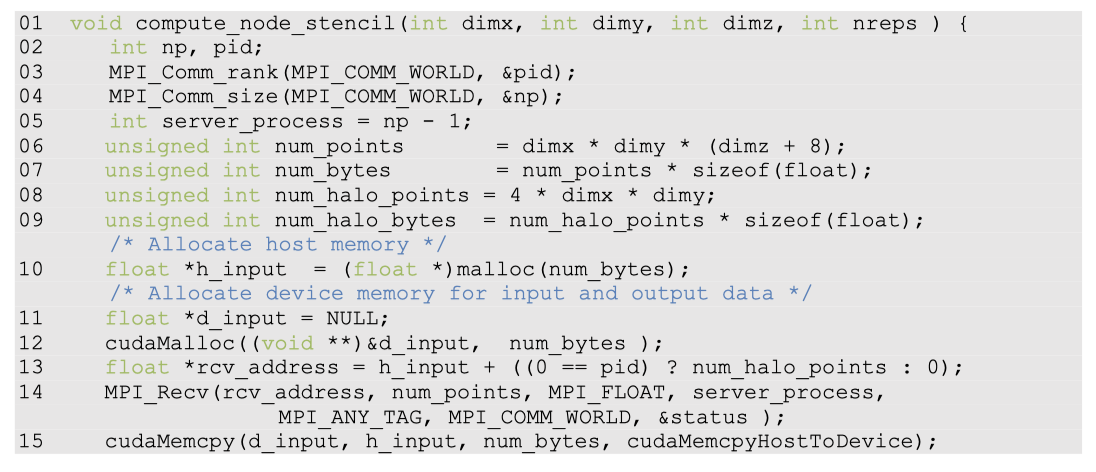
\includegraphics[width=0.9\textwidth]{figs/F20.10.png}
	\caption{\textit{计算进程代码(第 1 部分)。}}
\end{figure}

现在,我们将注意力转向从数据服务器进程接收输入的计算进程。 
在图 20.10 中,第 03-04 行建立了进程的进程 ID 以及应用程序的进程总数。 第 05 行确定数据服务器是进程 np -1 。 
$06-07$ 行计算网格点的数量以及每个内部进程应处理的字节数。 $08-09$ 行计算网格点的数量和每个光环(4 个切片)中的字节数。

第 10-12 行为输入数据分配主机内存和设备内存。 
尽管边缘进程需要较少的 halo 数据,但为了简单起见,它们仍然分配相同数量的内存; 部分分配的内存将不会被边缘进程使用。 
第13行设置主机存储器的起始地址,用于接收来自数据服务器的输入数据。 
对于除进程 0 之外的所有计算进程,起始接收位置只是为输入数据分配的内存的起始位置。 
然而,对于进程 0 ,我们将接收位置调整了四个切片。 
这是因为为了简单起见,我们假设用于接收输入数据的主机内存对于所有计算进程都以相同的方式排列:来自左邻居的四个光环元素切片,
后面跟着分区,然后是来自左邻居的四个光环元素切片。 正确的邻居。 
然而,正如我们在图 20.9 的第 15 行中所示,数据服务器不会将任何来自左邻居的光环数据发送到进程 0 。 
也就是说,对于进程 0 ,来自数据服务器的 MPI 消息仅包含来自右邻居的分区和光环。 
因此,第 13 行将起始主机内存位置调整了四个片,以便进程 0 能够正确解释来自数据服务器的输入数据。

第 14 行接收来自数据服务器的 MPI 消息。 大多数参数应该是熟悉的。 最后一个参数反映了接收数据时发生的任何错误情况。 
第二个参数指定所有计算进程将从数据服务器接收全部数据。 
然而,数据服务器将发送较少的数据到进程 0 和进程 $\mathrm{np}$ -2 。 
这没有反映在代码中,因为 MPI\_Recv() 允许第二个参数指定比实际接收到的数据点数量更多的数据点,
并且只会将从发送方接收到的实际字节数放入接收内存中。 
在进程 0 的情况下,来自数据服务器的输入数据仅包含来自右邻居的分区和光环。 
接收到的输入将通过跳过已分配内存的前四个切片来放置,这些切片对应于(不存在的)左邻居的光环。 
这种效果是通过第 13 行的术语 ( $(0==p i d)$ ? num\_halo\_points: 0$)$ 来实现的。
在进程 $n p-2$ 的情况下,输入数据包含来自 左邻居和分区。 
接收到的输入将从已分配内存的开头放置,而已分配内存的最后四个片未使用。

第 15 行将接收到的输入数据复制到设备内存中。 在过程 0 的情况下,左晕点无效。 在过程 $n p-2$ 的情况下,右侧光环点无效。 
但是,为了简单起见,所有计算节点都会将完整大小发送到设备内存。 假设内核将以正确忽略这些无效部分的方式启动。 
第 15 行之后,所有输入数据都在设备内存中。

\begin{figure}[H]
	\centering
	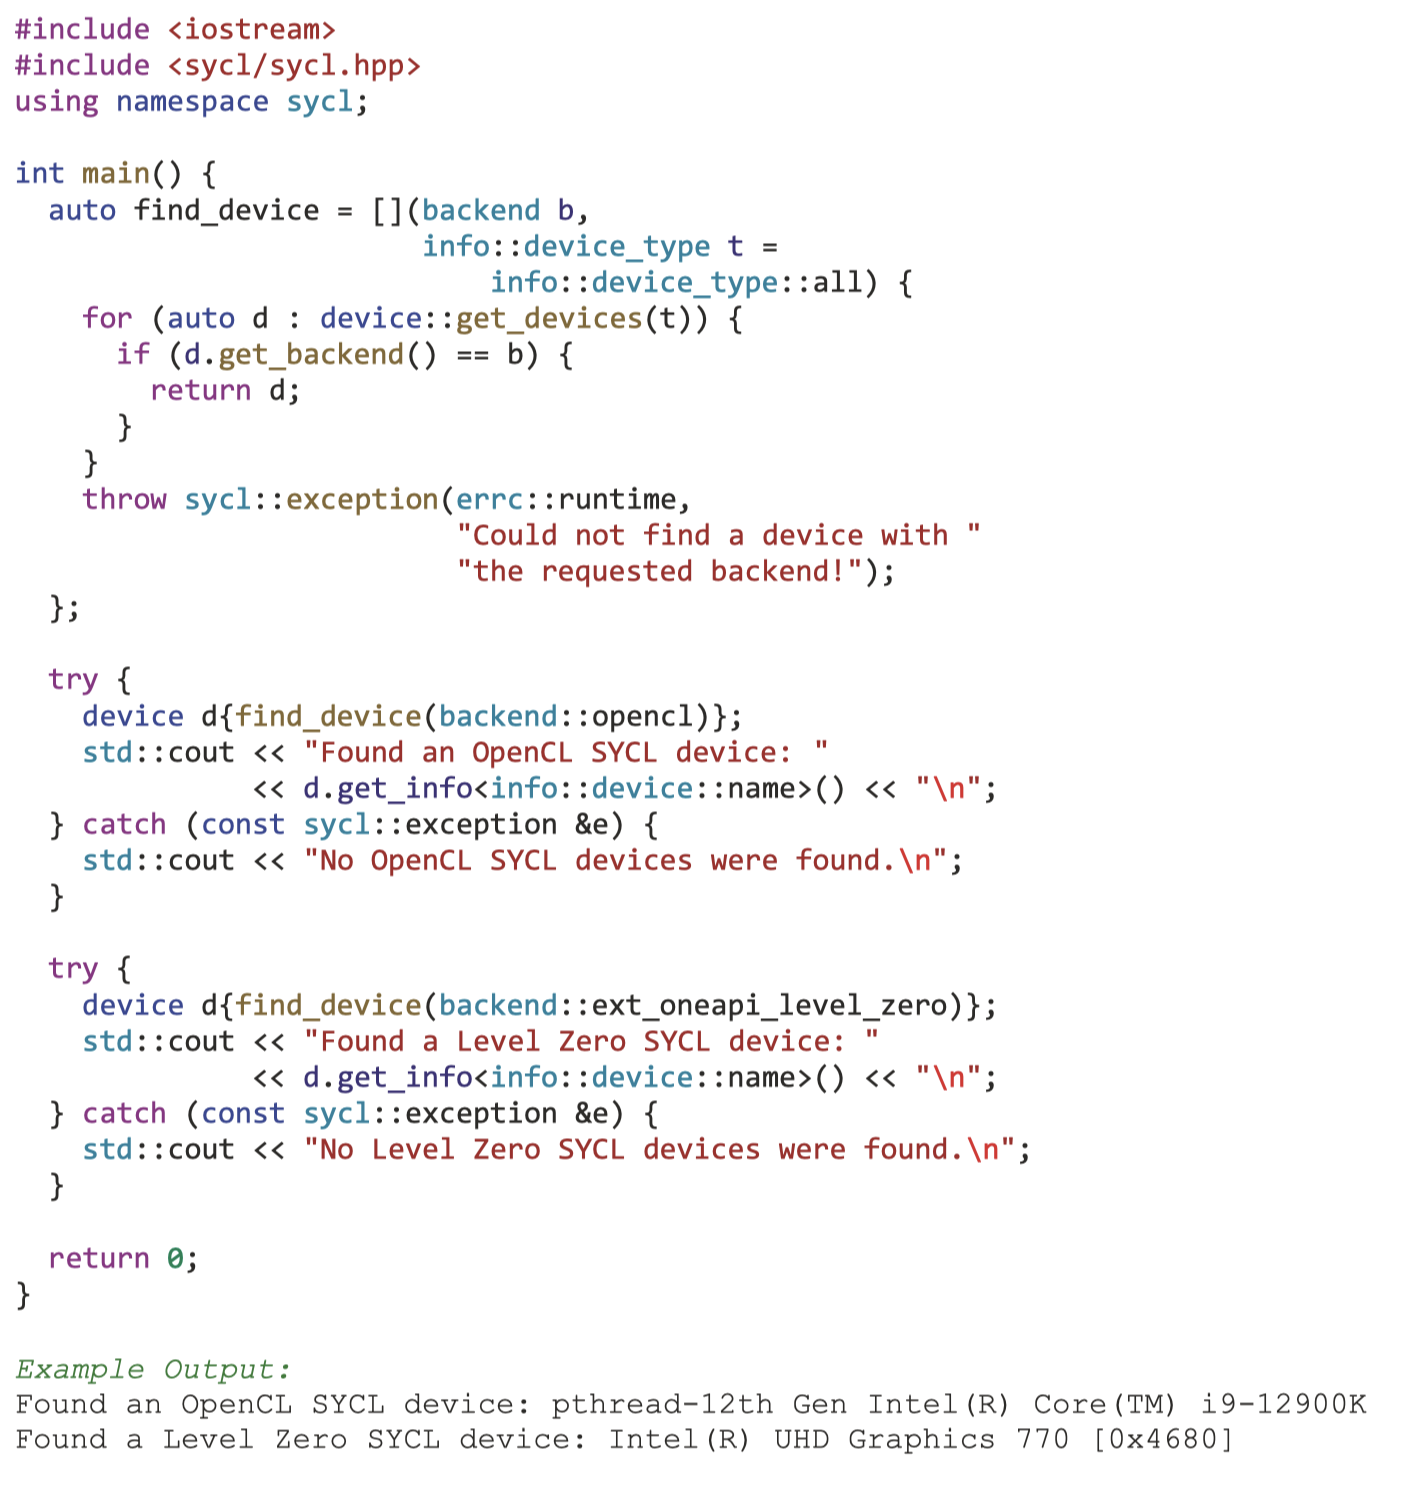
\includegraphics[width=0.9\textwidth]{figs/F20.11.png}
	\caption{\textit{计算进程代码(第 2 部分)。}}
\end{figure}

图 20.11 显示了计算过程代码的第 2 部分。 第 16-18 行为输出数据分配主机内存和设备内存。 
设备存储器中的输出数据缓冲区将与双缓冲方案中的输入数据缓冲区一起使用。 
也就是说,他们会在每次迭代中切换角色。 稍后我们将回到这一点并介绍图 20.11 中的其余代码。 
我们现在准备好展示在网格点上执行计算步骤的代码。

\subsection{重叠计算和通信}
\begin{figure}[H]
	\centering
	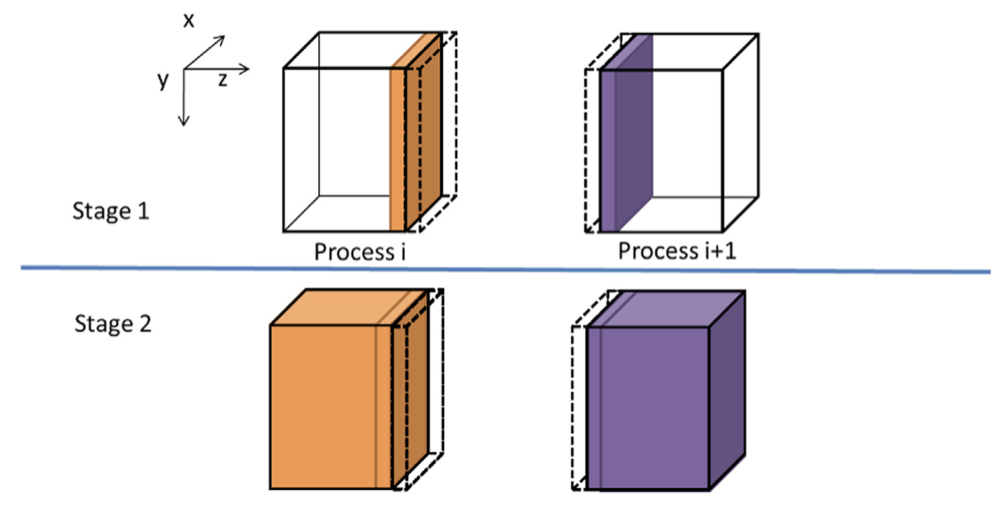
\includegraphics[width=0.9\textwidth]{figs/F20.12.png}
	\caption{\textit{重叠计算与通信的两阶段策略。}}
\end{figure}

执行计算步骤的一种简单方法是每个计算进程在其整个分区上执行计算步骤,与左右邻居交换光环数据,然后重复。 
虽然这是一个非常简单的策略,但并不是很有效。 原因是该策略迫使系统处于两种模式之一。 
在第一种模式中,所有计算进程都执行计算步骤。 在此期间,不使用通信网络。 
在第二种模式下,所有计算进程都与其左右邻居交换光环数据。 在此期间,计算硬件没有得到很好的利用。 
理想情况下,我们希望始终利用通信网络和计算硬件来实现更好的性能。 
这可以通过将每个计算过程的计算任务分为两个阶段来实现,如图20.12所示。

在第一阶段(第 1 阶段)期间,每个计算进程都会计算其边界切片,在下一次迭代中,其邻居将需要这些边界切片作为光环单元。 
我们继续假设我们使用四片光环数据。 图 20.12 将四个光环切片显示为虚线透明块,将四个边界切片显示为彩色块。 
请注意,进程 $i$ 的彩色部分将被复制到进程 $I+1$ 的虚线部分,
并且进程 $I+1$ 的彩色部分将在下一个过程中被复制到进程 $i$ 的虚线部分。 
沟通。 对于过程 0 ,第一阶段计算边界数据的右侧四个切片。 对于内部节点,它计算其边界数据的左侧四个切片和右侧四个切片。 
对于进程$n-2$,它计算其边界数据的左四部分。 基本原理是这些边界切片是其邻居下一次迭代所需要的。 
如果首先计算这些边界切片,则可以将数据传送给邻居,同时计算进程计算其内部网格点的其余部分。

在第二阶段(阶段 2),每个计算进程并行执行两项活动。 第一个是将其新边界值传达给其邻居进程。 
这是通过首先将数据从设备内存复制到主机内存,然后向邻居发送 MPI 消息来完成的。 
正如我们稍后将讨论的,我们需要注意从邻居接收的数据用于下一次迭代,而不是当前迭代。 第二个活动是计算分区中的其余数据。 
如果通信活动比计算活动花费的时间短,我们就可以隐藏通信延迟并始终充分利用计算硬件。 
这通常是通过在每个分区的内部拥有足够的切片来实现的,以允许每个计算进程执行足够的计算来隐藏通信。

为了支持第 2 阶段的并行活动,我们需要使用 CUDA 编程模型的两个高级功能:固定内存分配和流。 
固定内存分配请求所分配的内存不被操作系统调出。 这是通过 cudaHostAlloc() API 调用完成的。 
图 20.11 中的第 21-24 行为左右边界切片和左右光晕切片分配固定内存缓冲区。 
左边界切片和右边界切片需要从设备内存发送到左邻居进程和右邻居进程。 
这些缓冲区用作设备将数据复制到其中的主机内存暂存区域,然后用作 MPI\_Send() 到相邻进程的源缓冲区。 
左、右晕圈切片需要从相邻进程接收。 
这些缓冲区用作 MPI\_Recv() 的主机内存暂存区域,以用作目标缓冲区,然后将数据从其中复制到设备内存。 
这些缓冲区有时称为反弹缓冲区,因为它们的主要作用是充当临时缓冲区,允许数据从设备内存反弹到远程 MPI 进程,反之亦然。 
请注意,反弹缓冲区的主机内存分配是通过 cudaHostAlloc() 函数而不是标准 malloc() 函数完成的。 
不同之处在于 cudaHostAlloc() 函数分配固定内存缓冲区,有时也称为页锁定内存缓冲区。 
我们需要了解更多有关操作系统内存管理的背景知识,才能充分理解固定内存缓冲区的概念。

在现代计算机系统中,操作系统管理应用程序的虚拟内存空间。 每个应用程序都可以访问大的、连续的地址空间。 
实际上,系统的物理内存数量有限,需要在所有正在运行的应用程序之间共享。 
这种共享是通过将虚拟内存空间划分为页面并仅将活跃使用的页面映射到物理内存来执行的。 
当内存需求较多时,操作系统需要将部分页面从物理内存调出到大容量存储(例如磁盘)。 
因此,应用程序可以在执行期间随时将其数据调出。

cudaMemcpy() 的实现使用一种称为直接内存访问 (DMA) 设备的硬件。 
当调用 cudaMemcpy() 函数在主机和设备内存之间进行复制时,其实现使用 DMA 操作来完成任务。 
在主机内存方面,DMA硬件对物理地址进行操作; 也就是说,操作系统需要给DMA设备一个翻译后的物理地址。 
然而,数据有可能在 DMA 操作完成之前被调出。 数据的物理存储器位置可以被重新分配给与不同虚拟存储器位置相对应的其他数据。 
在这种情况下,DMA 操作可能会被损坏,因为其数据可能会被分页活动覆盖。

此数据损坏问题的常见解决方案是让 CUDA 运行时分两步执行复制操作。 
对于主机到设备的复制,CUDA 运行时首先将源主机内存数据复制到固定内存缓冲区中,
这意味着内存位置已标记,以便分页机制不会分页数据。 然后,它使用 DMA 设备将数据从固定内存缓冲区复制到设备内存。 
对于设备到主机的复制,CUDA 运行时首先使用 DMA 设备将数据从设备内存复制到固定内存缓冲区中。 
然后,它将数据从固定内存缓冲区复制到目标主机内存位置。 
通过使用额外的固定内存缓冲区,DMA 副本将不会受到任何分页活动的影响。

这种方法有两个问题。 一是额外的副本会增加 cudaMemcpy() 操作的延迟。 
第二个是所涉及的额外复杂性导致 cudaMemcpy() 函数的同步实现。 
也就是说,在 cudaMemcpy() 函数完成其操作并返回之前,主机程序无法继续执行。 
这会序列化所有复制操作。 为了支持具有更多并行性的快速复制,CUDA 提供了 cudaMemcpyAsync() 函数。

cudaMemcpyAsync() 函数要求将主机内存缓冲区分配为固定内存缓冲区。 
这是在图 20.11 中的第 21-24 行中针对左边界、右边界、左光环和右光环切片的主机存储器缓冲区完成的。 
这些缓冲区是使用 cudaHostAlloc() 函数分配的,这确保分配的内存被固定或页面锁定以防止分页活动。 
请注意,cudaHostalloc() 函数采用三个参数。 前两个与 cudaMalloc() 相同。 
第三个指定了一些更高级用法的选项。 对于大多数基本用例,我们可以简单地使用默认值 cudaHostAllocDefault。

用于与计算重叠通信的第二个高级 CUDA 功能是流,该功能支持 CUDA API 函数的托管并发执行。 流是一个有序的操作序列。 
当主机代码调用 cudaMemcpyAsync() 函数或启动内核时,它可以指定一个流作为其参数之一。 
通过在 cudaMemcpyAsync() 调用中指定流,复制操作将被放入流中。 同一流中的所有操作将根据它们放入该流的顺序依次完成。 
然而,不同流中的操作可以并行执行,没有任何顺序约束。

图 20.11 的第 25 行声明了两个 CUDA 内置类型 cudaStream\_t 的变量。 
然后使用这些变量来调用 cudaStreamcreate() 函数。 
每次调用 cudaStreamcreate() 都会创建一个新流并将该流的标识符存入其参数中。 
在第 26 行和第 27 行中的调用之后,主机代码可以在后续的 cudaMemcpyAsync() 调用和内核调用中使用流 0 或流 1。

\begin{figure}[H]
	\centering
	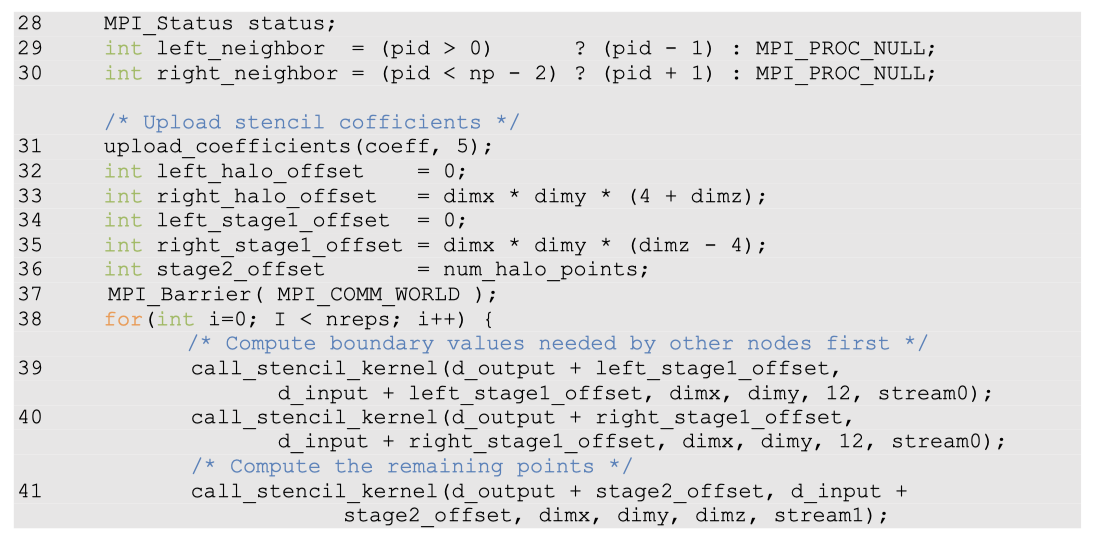
\includegraphics[width=0.9\textwidth]{figs/F20.13.png}
	\caption{\textit{计算进程代码(第 3 部分)。}}
\end{figure}

图 20.13 显示了计算过程的第 3 部分。 第 28 行声明了一个将用于 MPI 发送和接收的 MPI 状态变量。 
第 29-30 行计算计算进程的左右邻居的进程 ID。 
当计算进程向邻居发送消息或从邻居接收消息时,左邻居和右邻居变量将被计算进程用作参数。 
对于进程 0 ,没有左邻居,因此第 29 行将 MPI 常量 MPI\_PROC\_NULL 分配给 1eft\_neighbor 来记录这一事实。 
对于进程 np - 2,没有右邻居,因此第 30 行将 MPI\_PROC\_NULL 分配给右\_邻居。 
对于所有内部进程,第 $29-30$ 行将 pid -1 分配给 left\_neighbor,将 pid +1 分配给 right\_neighbor。

图 20.13 中的第 31 行调用一个函数将模板系数复制到 GPU 常量内存。 这里不再展示细节,因为读者应该已经熟悉常量内存。 
第32-36行设置了几个偏移量,这些偏移量将用于调用内核和交换数据,以便计算和通信可以重叠。 
这些偏移量定义了需要在图 20.13 的每个阶段计算的网格点区域。 它们也在图 20.12 中进行了可视化。

\begin{figure}[H]
	\centering
	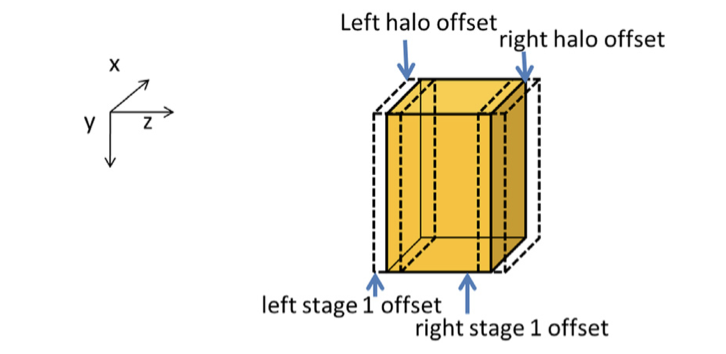
\includegraphics[width=0.9\textwidth]{figs/F20.14.png}
	\caption{\textit{用于与邻居进程交换数据的设备内存偏移量。}}
\end{figure}

请注意,每个设备内存中的切片总数为四片左晕点(白色虚线)
加上四片左边界点加上 dimx*dimy(dimz -8) 内部点加上四片右边界点 边界点加上四片右晕点(白色虚线)。 
如图 20.14 所示,变量 1eft\_stage1\_offset 定义了计算左边界切片所需的切片的起点。 
这包括 12 个数据切片:四个左邻居光晕点切片、四个边界点切片和四个内部点切片。 
这些切片位于分区的最左边,因此第 34 行将偏移值设置为 0。 
变量 right\_stage2\_offset 定义计算右边界切片所需的切片的起点。 
这还包括 12 个切片:四个内部点切片、四个右边界点切片和四个右晕环单元切片。 
这 12 个切片的起始点可以通过从切片总数 dimz +8 中减去 12 来得出。 
因此,这 12 个切片的起始偏移量在第 35 行设置为 dimx*dimy*(dimz-4)(图 20.12)。

图20.13中的第37行是MPI屏障同步,类似于块中跨线程的 CUDA \_\_syncthreads()。 
MPI 屏障强制由输入参数指定的所有 MPI 进程相互等待。 在所有进程都到达此点之前,没有任何进程可以继续执行超出此点的操作。 
我们在这里想要屏障同步的原因是为了确保所有计算节点都已收到其输入数据并准备好执行计算步骤。 
由于它们将相互交换数据,因此我们希望使它们全部在大约同一时间开始。 
因此,在数据交换期间,我们不会遇到少数迟缓进程延迟所有其他进程的情况。 
MPI\_Barrier() 是一个集体通信函数。 我们将在下一节中更详细地讨论集体通信 API 函数。

第 38 行启动一个执行计算步骤的循环。 对于每次迭代,每个计算过程将执行图 20.12 所示的两阶段过程的一个周期。 
第 39 行调用一个函数,该函数将在阶段 1 中生成左边界点的四个切片。 
我们假设该函数将设置网格配置并调用模板内核,该内核对网格点区域执行一个计算步骤,如第 8 章“模板”中所述。 
cal1\_stenci1\_kerne 1 () 函数有几个参数。 
第一个参数是指向内核输出数据区域的指针。 第二个参数是指向输入数据区域的指针。 
在这两种情况下,我们都会将 1eft\_stage1\_offset 添加到设备内存中的输入和输出数据中。 
接下来的三个参数指定要处理的网格部分的尺寸。 
请注意,我们需要在每侧有四个切片,以便正确地对四个左边界切片中的所有点执行计算。 
第 40 行对阶段 1 中的右边界点执行相同的操作。 请注意,这些内核将在流 0 中调用并按顺序执行。

第 41 行调用 ca11\_stenci1\_kernel() 函数,
该函数将调用模板内核函数来生成阶段 2 中的 dimx*dimy*(dimz-8) 内部点。 
请注意,这还需要每侧有四个输入边界值切片,因此输入切片的总数为 dimx*dimy*dimz。 
内核在流 1 中被调用,并将与第 39 行和第 40 行调用的内核并行执行。

\begin{figure}[H]
	\centering
	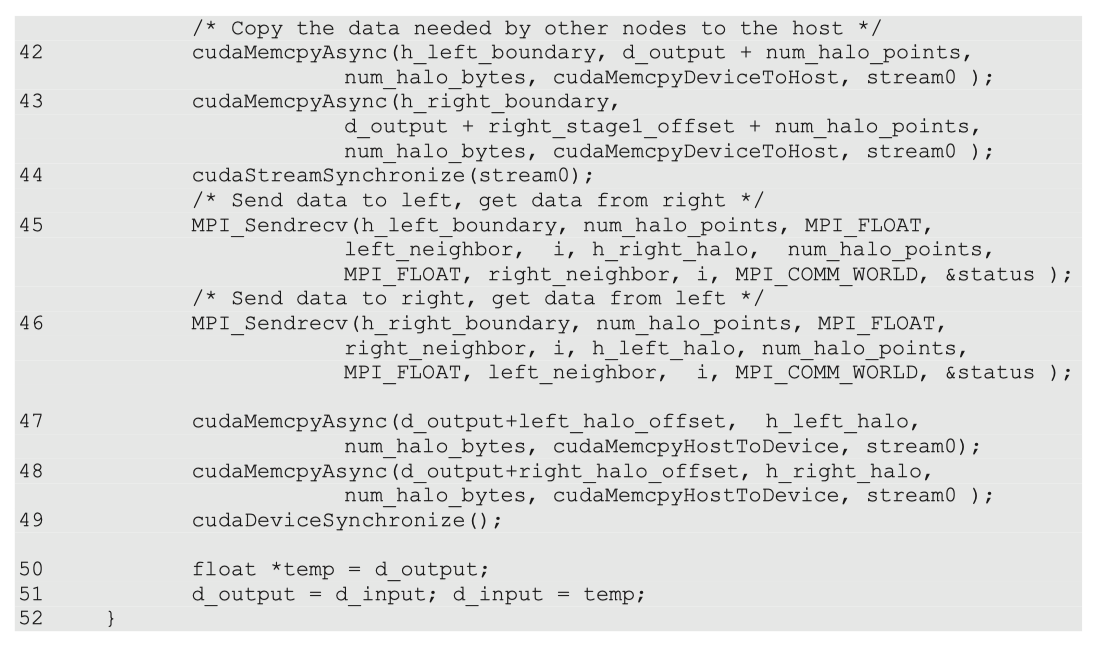
\includegraphics[width=0.9\textwidth]{figs/F20.15.png}
	\caption{\textit{计算进程代码(第 4 部分)。}}
\end{figure}

图 20.15 显示了计算过程代码的第 4 部分。 第 42 行将左边界点的四个切片复制到主机内存,准备与左邻居进程进行数据交换。 
第 43 行将右边界点的四个切片复制到主机内存,准备与右邻居进程进行数据交换。 
两者都是流 0 中的异步副本,并且将等待流 0 中的两个内核完成后才复制数据。 
第 44 行是同步,强制进程等待流 0 中的所有操作完成后才能继续。 
这确保了在进程继续进行数据交换之前左边界点和右边界点位于主机存储器中。

\begin{figure}[H]
	\centering
	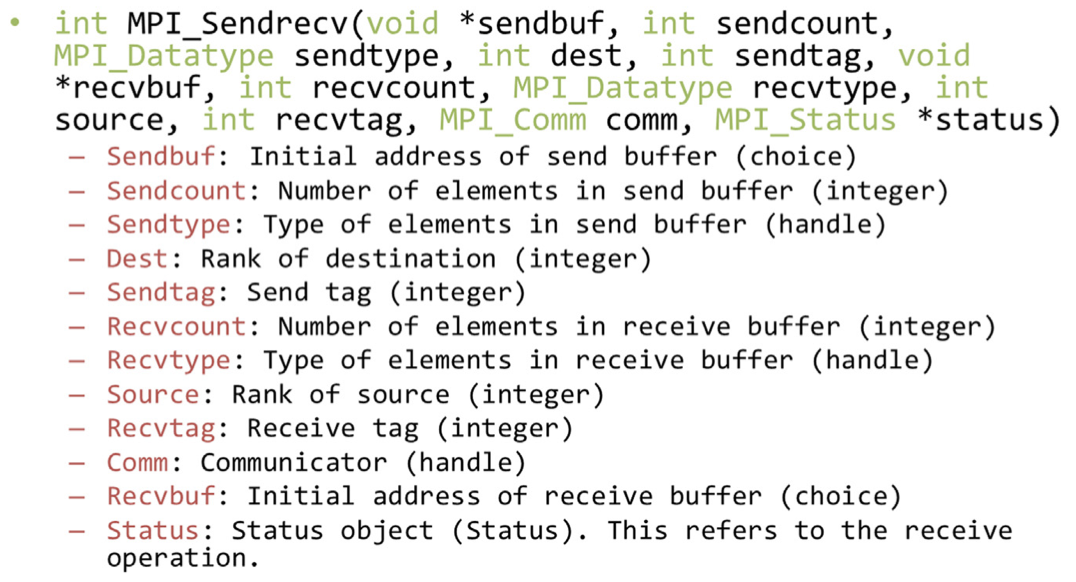
\includegraphics[width=0.9\textwidth]{figs/F20.16.png}
	\caption{\textit{MPI\_Sendrecv() 函数的语法。}}
\end{figure}

在数据交换阶段,我们将让所有 MPI 进程将其边界切片发送到其左邻居。 也就是说,所有进程都会有其正确的邻居向它们发送数据。 
因此,使用 MPI 函数将数据发送到目的地并从源接收数据会很方便。 这减少了 MPI 函数调用的数量。 
图20.16中的MPI\_Sendrecv()函数就是这样一个函数。 
它是 MPI\_Send() 和 MPI\_Recv() 的组合,因此我们不再详细说明参数的含义。

第 45 行将左边界点的四个切片发送到左邻居,并从右邻居接收右晕点的四个切片。 
第 46 行将四片右边界点发送到右邻居,并从左邻居接收四片左晕点。 
对于进程 0 ,其 1eft\_neighbor 在第 27 行中已设置为 MPI\_PROC\_NULL ,
因此 MPI 运行时不会为进程 0 发送第 45 行中的消息或接收第 46 行中的消息。 
同样,对于进程 $n p-2$,MPI 运行时不会接收第 45 行中的消息,也不会发送第 46 行中的消息。 
因此,图 20.13 的第 29 行和第 30 行中的条件赋值消除了第 45 行和第 46 行中对特殊 ifthen-else 语句的需要。

发送和接收 MPI 消息后,第 47 行和第 48 行将新接收到的光环点传输到设备内存的 d\_output 缓冲区。 
这些副本在流 0 中完成,因此它们将与第 38 行流 1 中启动的内核并行执行。

第49行是所有设备活动的同步操作。 此调用强制进程等待所有设备活动(包括内核和数据副本)完成。 
当 cudaDeviceSynchronize() 函数返回时,
当前计算步骤中的所有 d\_output 数据都已就位:来自左邻居进程的左晕数据、来自第 36 行启动的内核的边界数据、
来自第 38 行启动的内核的内部数据 ,来自第 37 行启动的内核的右边界数据,以及来自右邻居的右晕圈数据。

第 50 行和第 51 行交换了 d\_input 和 d\_output 指针。 
这会将当前计算步骤的 d\_ouput 数据的输出更改为下一个计算步骤的 d\_input 数据。 
然后,执行通过进入第 35 行循环的下一次迭代来进入下一个计算步骤。 
这将持续下去,直到所有计算进程都完成了参数 nreps 指定的计算次数。

\begin{figure}[H]
	\centering
	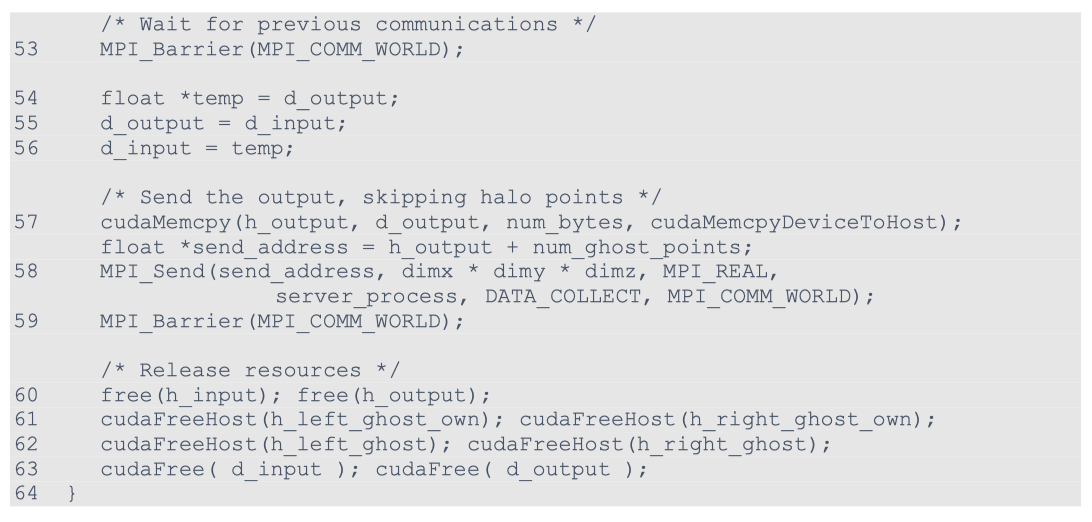
\includegraphics[width=0.9\textwidth]{figs/F20.17.png}
	\caption{\textit{计算进程代码(第 5 部分)。}}
\end{figure}

图 20.17 显示了第 5 部分,即计算过程代码的最后部分。 第 53 行是屏障同步,强制所有进程互相等待完成其计算步骤。 
第 54-56 行将 d\_output 与 d\_input 交换。 
这是因为第 50 行和第 51 行将 d\_output 与 d\_input 交换,为下一个计算步骤做准备。 
然而,这对于最后一个计算步骤是不必要的,因此我们使用第 54-56 行来撤消交换。 第 57 行将最终输出复制到主机内存。 
第 58 行将输出发送到数据服务器。 第 59 行等待所有进程完成。 第 60-63 行在返回主程序之前释放所有资源。

\begin{figure}[H]
	\centering
	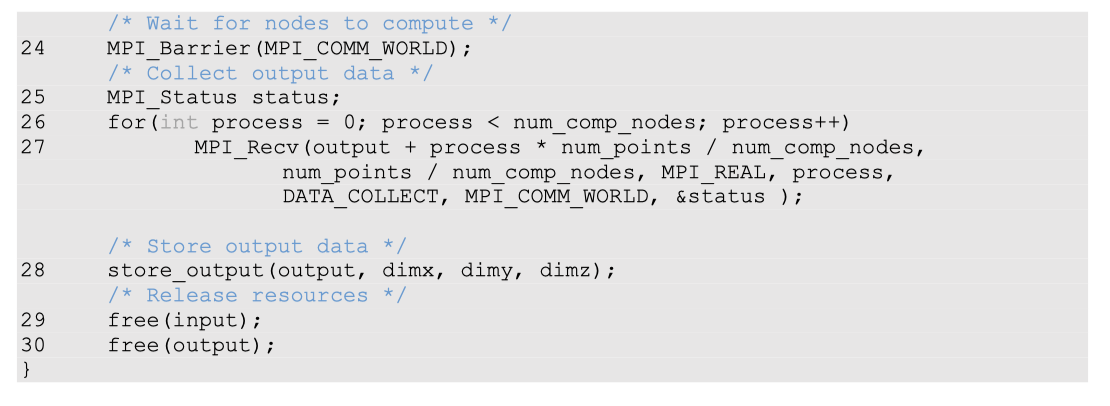
\includegraphics[width=0.9\textwidth]{figs/F20.18.png}
	\caption{\textit{数据服务器代码(第 2 部分)。}}
\end{figure}

图 20.18 显示了第二部分,即数据服务器代码的最后部分,是图 20.9 的延续。 
第 24 行是屏障同步,等待所有计算节点完成其计算步骤并发送其输出。 该屏障对应于计算过程第 59 行的屏障。 
第 26 行和第 27 行接收来自所有计算进程的输出数据。 第 28 行将输出存储到外部存储器中。 
最后,第 29 行和第 30 行在返回主程序之前释放资源。

\subsection{消息传递接口集体通信}
我们在上一节中看到了 MPI 集体通信 API 的示例:MPI\_Barrier。 
其他常用的群体集体通信类型是广播、减少、聚集和分散(Gropp 等,1999)。 
屏障同步 MPI\_Barrier() 也许是最常用的集体通信函数。 
正如我们在模板示例中看到的,屏障用于确保所有 MPI 进程在开始相互交互之前都已准备好。 
我们不会详细说明其他类型的 MPI 集体通信函数,但我们鼓励读者阅读这些函数的详细信息。 
一般来说,集体通信功能由 MPI 运行时开发人员和系统供应商进行了高度优化。 
与尝试通过发送和接收调用的组合来实现相同的功能相比,使用它们通常会带来更好的性能、可读性和生产力。

\subsection{CUDA 感知消息传递接口}
现代 MPI 实现了解 CUDA 编程模型,旨在最大限度地减少 GPU 之间的通信延迟。 
目前,MVAPICH2、IBM Platform MPI 和 OpenMPI 支持 CUDA 和 MPI 之间的直接交互。

CUDA 感知的 MPI 实现能够将消息从一个节点中的 GPU 内存发送到另一节点中的 GPU 内存。 
这有效地消除了在发送 MPI 消息之前进行设备到主机数据传输以及在接收 MPI 消息之后进行主机到设备数据传输的需要。 
这有可能简化主机代码和内存数据布局。 
在我们的模板示例中,如果我们使用 CUDA 感知的 MPI 实现,我们将不再需要主机固定的内存分配和异步内存复制。

第一个简化是我们不再需要分配主机固定的内存缓冲区来将光环点传输到主机内存来为 MPI\_Send( ) 做准备。 
这意味着我们可以安全地删除图 20.11 中的第 21-24 行。 
然而,我们仍然需要使用 CUDA 流和两个独立的 GPU 内核,以便在计算光环元素后立即开始跨节点通信。

\begin{figure}[H]
	\centering
	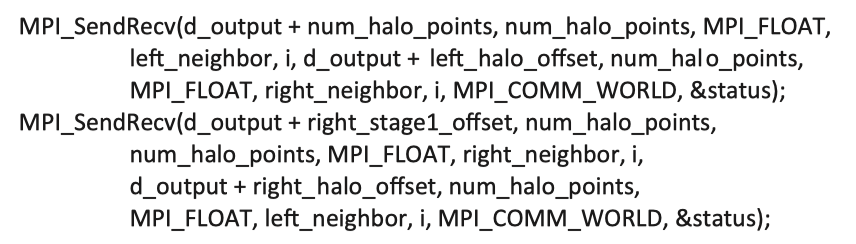
\includegraphics[width=0.9\textwidth]{figs/F20.19.png}
	\caption{\textit{使用 CUDA-aware MPI 修订了 MPI SendRecv 调用。}}
\end{figure}

第二个简化是我们不再需要在 MPI\_Recv() 之后将 halo 数据从主机异步复制到设备内存。 
因此,我们还可以删除图 20.15 中的第 42 行和第 43 行。 
由于 MPI 调用现在接受设备内存地址,因此我们需要修改对 MPI\_SendRecv 的调用才能使用它们。 
注意,这些内存地址实际上对应于之前版本中异步内存副本的设备地址。 
由于 CUDA 感知的 MPI 实现将直接更新 GPU 内存的内容,因此我们还删除了图 20.15 中的第 47 行和第 48 行。 
图20.19显示了对图20.15中第45行和第46行中的MPI\_SendRecv语句的修改,以便它们直接从设备存储器中读取和写入。

除了使用 MPI\_SendRecv() 删除光环交换期间的数据传输之外,
还可以通过直接从 GPU 内存接收/发送输入/输出来删除初始和最终内存副本。

\subsection{总结}
在本章中,我们介绍了具有异构计算节点的 HPC 集群的 CUDA/MPI 联合编程的基本模式。 
MPI 应用程序中的所有进程都运行相同的程序。 
但是,每个进程可以遵循不同的控制流和函数调用路径来专门化其角色,如我们示例中的数据服务器和计算进程所示。 
我们还使用模板模式来展示计算过程如何交换数据。 我们提出了使用 CUDA 流和异步数据传输来实现计算和通信的重叠。 
我们还展示了如何使用 MPI 屏障来确保所有进程都准备好相互交换数据。 
最后,我们简要概述了使用 CUDA 感知 MPI 来简化设备内存中的数据交换。 
我们想指出,虽然 MPI 是一个非常不同的编程系统,但我们在本章中介绍的所有主要 MPI 概念,即 SPMD、MPI 等级和障碍,
在 CUDA 编程模型中都有对应的概念。 
这证实了我们的信念:通过使用一种模型很好地教授并行编程,我们的学生可以快速轻松地掌握其他编程模型。 
我们希望鼓励读者在本章提供的基础上学习更高级的 MPI 功能和其他重要模式。